%%%%%%%%%%%%%%%%%%%%%%%%%%%%%%%%%%%%%%%%%%%%%%%
%%% Template for lab reports used at STIMA
%%%%%%%%%%%%%%%%%%%%%%%%%%%%%%%%%%%%%%%%%%%%%%%

%%%%%%%%%%%%%%%%%%%%%%%%%%%%%% Sets the document class for the document
% Openany is added to remove the book style of starting every new chapter on an odd page (not needed for reports)
\documentclass[10pt,english, openany]{book}

%%%%%%%%%%%%%%%%%%%%%%%%%%%%%% Loading packages that alter the style
\usepackage[]{graphicx}
\usepackage[]{color}
\usepackage{alltt}
\usepackage[T1]{fontenc}
\usepackage[utf8]{inputenc}
\setcounter{secnumdepth}{3}
\setcounter{tocdepth}{3}
\setlength{\parskip}{\smallskipamount}
\setlength{\parindent}{0pt}
\usepackage{biblatex}
\addbibresource{bibliography.bib}
% Set page margins
\usepackage[top=100pt,bottom=100pt,left=68pt,right=66pt]{geometry}

% Package used for placeholder text
\usepackage{lipsum}

% Prevents LaTeX from filling out a page to the bottom
\raggedbottom

% Adding both languages
\usepackage[english, italian]{babel}

% All page numbers positioned at the bottom of the page
\usepackage{fancyhdr}
\fancyhf{} % clear all header and footers
\fancyfoot[C]{\thepage}
\renewcommand{\headrulewidth}{0pt} % remove the header rule
\pagestyle{fancy}

% Changes the style of chapter headings
\usepackage{titlesec}
\titleformat{\chapter}
   {\normalfont\LARGE\bfseries}{\thechapter.}{1em}{}
% Change distance between chapter header and text
\titlespacing{\chapter}{0pt}{50pt}{2\baselineskip}

% Adds table captions above the table per default
\usepackage{float}
\floatstyle{plaintop}
\restylefloat{table}



% Adds space between caption and table
\usepackage[tableposition=top]{caption}

% Adds hyperlinks to references and ToC
\usepackage{hyperref}
\hypersetup{hidelinks,linkcolor = black} % Changes the link color to black and hides the hideous red border that usually is created

% If multiple images are to be added, a folder (path) with all the images can be added here 
\graphicspath{ {Figures/} }

% Separates the first part of the report/thesis in Roman numerals
\frontmatter

\usepackage{graphicx}
\usepackage{caption}
\usepackage{float}

% no page break
\newenvironment{absolutelynopagebreak}
  {\par\nobreak\vfil\penalty0\vfilneg
   \vtop\bgroup}
  {\par\xdef\tpd{\the\prevdepth}\egroup
   \prevdepth=\tpd}

%%%%%%%%%%%%%%%%%%%%%%%%%%%%%% Starts the document
\begin{document}

%%% Selects the language to be used for the first couple of pages
\selectlanguage{english}

%%%%% Adds the title page
\begin{titlepage}
	\clearpage\thispagestyle{empty}
	\centering
	\vspace{1cm}

	% Titles
	% Information about the University
	{\normalsize Data Science and Economics \\ 
    Department of Economics, Management and Quantitative Methods\\
    Department of Computer Science "Giovanni degli Antoni"\\
		Università degli Studi di Milano\par}
		\vspace{3cm}
	{\Huge \textbf{Image classification with \\  Machine Learning: 	\vspace{0.5cm}
 }} \\
	{\large \textbf{recognising fruit and vegetable classes with Neural Networks}} \\
	%\vspace{1cm}
	%{\large \textbf{xxxxx} \par}
	\vspace{3cm}
	{\normalsize IERARDI ANDREA - 960188 \\ 	\vspace{0.5cm} % \\ specifies a new line
	             MORALES EMANUELE - 941935 \\	\vspace{0.5cm}
	             SAPORITO GREGORIO - 941503 \par}
	\vspace{3cm}
    
    \centering 
\includegraphics[scale=0.14]{logo.png}
    
    \vspace{0.5cm}
		
	% Set the date
	{\normalsize a.y. 2019/2020 \par}
	
	\pagebreak

\end{titlepage}
\newpage
\textit{We declare that this material, which We now submit for assessment, is entirely our own work and has not been taken from the work of others, save and to the extent that such work has been cited and acknowledged within the text of our work. We understand that plagiarism, collusion, and copying are grave and serious offences in the university and accept the penalties that would be imposed should I engage in plagiarism, collusion or copying. This assignment, or any part of it, has not been previously submitted by us or any other person for assessment on this or any other course of study.}

\vspace{3cm}

\textbf{Link to the repository}: \\ \href{https://github.com/Andreaierardi/Fruits-Neural-Networks/blob/master/project_code.ipynb}{https://github.com/Andreaierardi/Fruits-Neural-Networks/blob/master/project\_code.ipynb}
% Adds a table of contents
\tableofcontents{}
\listoffigures
%%%%%%%%%%%%%%%%%%%%%%%%%%%%%%%%%%%%%%%%%%%%%%%%%%%%%%%%%%%%%%%%%%%%%%%%%%%%%%%%%%%%%%%%%%%%
%%%%%%%%%%%%%%%%%%%%%%%%%%%%%%%%%%%%%%%%%%%%%%%%%%%%%%%%%%%%%%%%%%%%%%%%%%%%%%%%%%%%%%%%%%%%
%%%%% Text body starts here!
\mainmatter
\chapter{Summary}\label{chapt:sum}


The aim of the project is to train neural networks for the classification of fruit and vegetables by using Tensorflow. The dataset is retrieved from the online community Kaggle\footnote{\href{https://www.kaggle.com/moltean/fruits}{https://www.kaggle.com/moltean/fruits}}.

This work wants to explore different neural network techniques that are used for image classification, looking for the best architecture that solves the problem of fruit and vegetables recognition.

%The main points that inspire this work are the following:
The main questions addressed in this work are:

\begin{itemize}
\item How does the accuracy of the neural networks change by varying the complexity of the model?

\item Are mainstream architectures (i.e. LeNet and MobileNetV2) always reliable in order to solve image recognition problems?
\end{itemize}

Trying to answer these questions, the work consists of three main parts:

In the first part, feed forward neural networks are implemented.
Since these type of networks are less complex, the idea is to give them
as input a "simplified" problem and observe if the networks' performance is satisfactory.
The techniques used to reduce the complexity of the training set are:
\begin{itemize}
\item Conversion of the images from RGB to grayscale;		
	
\item Principal Component Analysis which allows to reduce the noise in the data.
\end{itemize}

The result of these two data manipulation techniques is given as input to a one-hidden-layer feed forward architecture.

The aim of this first part of the project is to study how the accuracy of the training, validation and test changes as the number of components
given as input increase.


In the second part, another type of neural-network which is notoriously more reliable for image recognition than an ordinary feed-forward architecture is inspected: Convolutional Neural Networks (CNN). 
As opposed to feed-forward NNs, CNNs receive as input tensors 
and use more operations, like convolution and pooling, that oftentimes result in a more precise classification.
In particular, the architecture used in this project is inspired by VGG net\footnote{VGG was introduced in 2014 by Andrew Zisserman and Karen Simonyan from the Oxford Robotics Institute}, at the moment one of the most used image-recognition architectures. For the purpose of this project, we start off with a small network and progressively increase the number of layers evaluating the change in performance and the potential overfitting
as the network becomes larger and more complex. To prevent overfitting, a series of techniques such as Dropout and Batch normalization are used.

In the last part of the project, two famous architectures in the machine learning literature are applied
to verify how the accuracy changes by using these consolidated architectures and compare their performance and the possible complications due to the complexity of the networks.
Specifically, the architectures applied in this section are LeNet and MobileNetV2.

\chapter{Preprocessing}
After downloading the data, the image size is reduced to 32x32 and the pixels are rescaled in a 0-1 range (dividing each value by 255). Subsequently, for each of the fruit labels a discrete value from 0 to 9 is assigned.

What follows is a visualisation of the first ten images from the training set.

\begin{figure}[h]
    \centering
    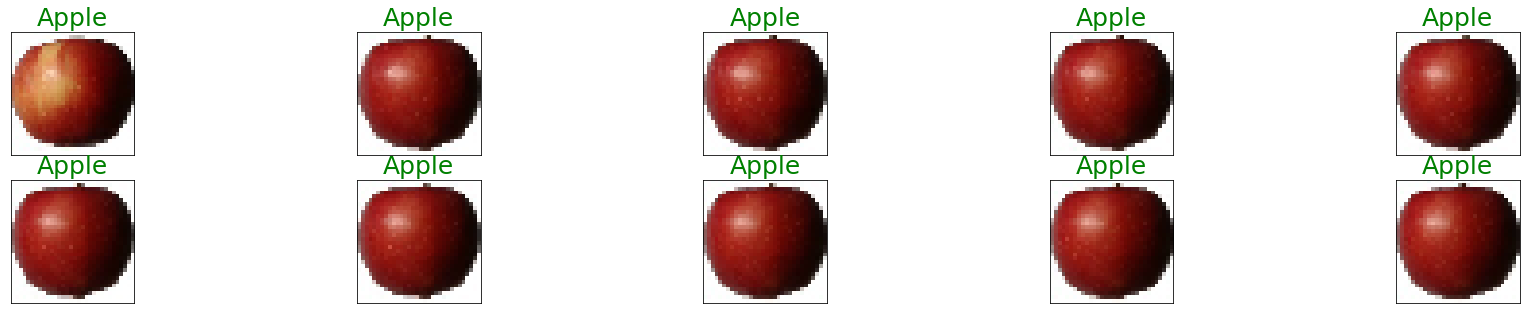
\includegraphics[width=0.9\textwidth]{Images/0.1. Visualisation of the first 10 images.png}
    \caption{ First 10 images from training set}
\end{figure}

The data is reshuffled to introduce randomisation in the training process (Figure \ref{fig:2.2}) and ensure that each fruit has a similar representation in the training, validation, and test sets.

\begin{figure}[h]
    \centering
    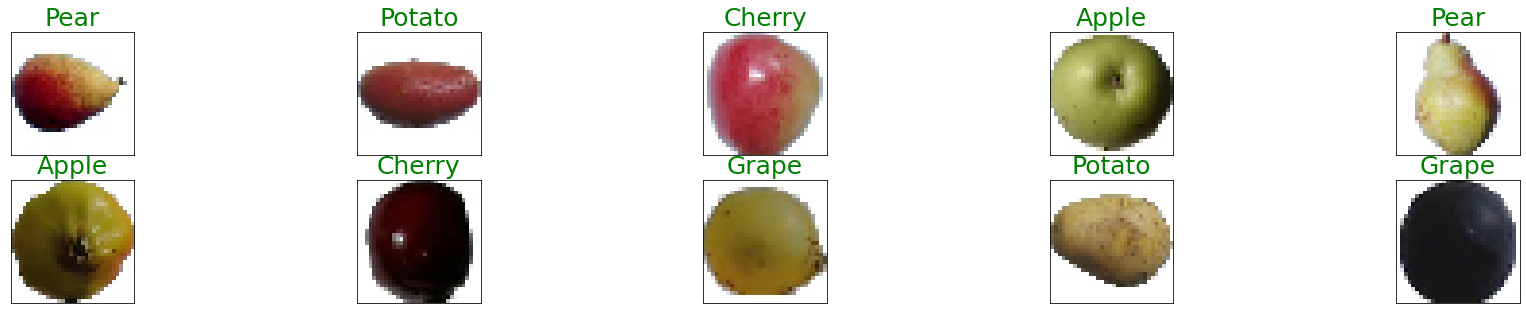
\includegraphics[width=0.9\textwidth]{Images/0.2.Visualisation 10 images shuffled.png}
    \caption{\label{fig:2.2}Shuffled images}
\end{figure}

The validation-test split of the image set is performed according to the 80\%-20\% criterion.
At the end of the process the train, validation, test split consists of:
\begin{itemize}
    \item Train X :  (32607, 32, 32, 3)
    \item Train y : (32607, 10)
    \item Validation X :  (8724, 32, 32, 3)
    \item Validation y : (8724, 10)
    \item Test X :  (2182, 32, 32, 3)
    \item Test y :  (2182, 10)
\end{itemize}

\chapter{Loss and activation functions used}
In all the architectures implemented, the algorithm is trained using the categorical cross-entropy. The optimizer used to train the network is \textit{Adam} and the main activation function \textit{Relu}. \textit{Relu} is chosen because, at an empirical level, it is one of the most popular among researchers.
To assess the final performance on the test set, however, the zero-one loss is used instead.

\begin{figure}[h]
    \centering
    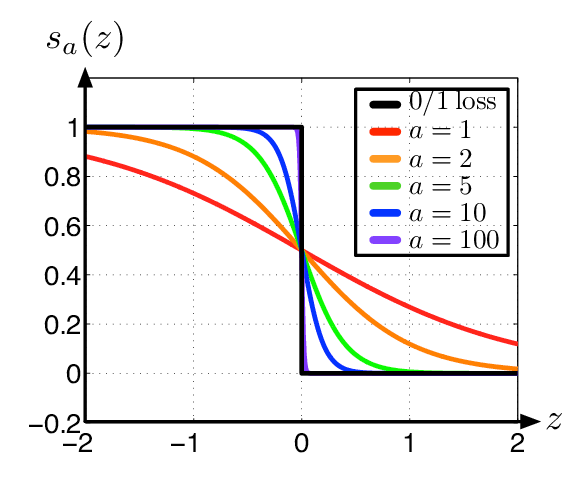
\includegraphics[width=0.5\textwidth]{Images/zero-one loss.png}
    \caption{\label{fig:3.1} Zero-one loss (black line)}
\end{figure}


\begin{figure}[h]
    \centering
    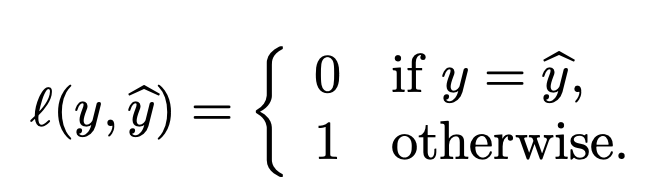
\includegraphics[width=0.3\textwidth]{Images/zero formula.png}
\end{figure}

\chapter{PCA and Feed-Forward Neural Networks}\label{chapt:doe}

\section{Greyscale and PCA}
Before running the PCA decomposition, the images are converted to grey scale attributing to each color a weight based on its different wavelenght.
$$
\textit{New grayscale image} = (0.3 \cdot R) + (0.59 \cdot G) + (0.11 \cdot B)
$$

The original shape of the image is a 32x32x3 tensor while the transformed one is a 32x32 matrix.

\begin{figure}[h]
  \centering
  \begin{minipage}[b]{0.48\textwidth}
    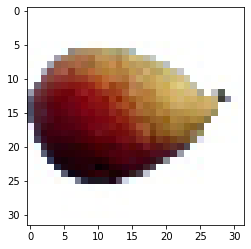
\includegraphics[width=0.7\textwidth]{Images/1.1.1 Pca and feed forward NN color.png}
    \caption{RGB image (32x32x3 format)}
  \end{minipage}
  \hfill
  \begin{minipage}[b]{0.48\textwidth}
    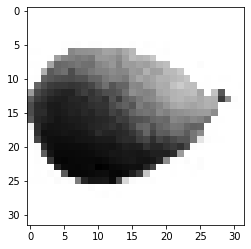
\includegraphics[width=0.7\textwidth]{Images/1.1.2 PCA and FFNN greyscale.png}
    \caption{Grayscale image (32x32)}
  \end{minipage}
\end{figure}

The resulting images are linearised from a 32x32 pixel matrix to a 1024 components vector. All the images are then combined into a matrix where each column corresponds to a single image and each row represents the corresponding pixel values. Then standardisation is applied using the following formula:

\begin{figure}[H]

    \centering
    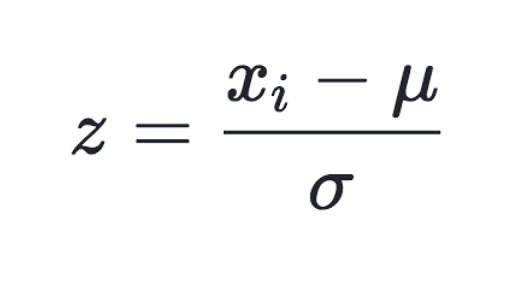
\includegraphics[width=0.18\textwidth]{Images/normalization.png}
\end{figure}

\newpage
The principal component decomposition is run starting from the covariance matrix. To figure out the number of principal components to reduce the noise in the images and then give them as input to a feed forward NN, a cumulative explained variance ratio analysis is computed (Figure \ref{fig:4.3}). This approach allows to reduce the noise in the data while retaining a sufficient percentage of explained variance that allows the algorithm to effectively discriminate between categories.
As can be seen from Figure \ref{fig:4.3}, a low number of components already explains a large part of the variance in the data.
For example, just by using 50 components 95 percent of the variance can already be explained.

This means that a marginal increase in the number of components in the model gives a minimal contribution when the number of components selected is already high (i.e. close to 1024); that is PCA can be used to simplify the problem.

For this reason only a range of components from 10 to 210 are considered with a step of 20 (i.e. 10,30,...,210). \\
\begin{figure}[H]
    \centering
    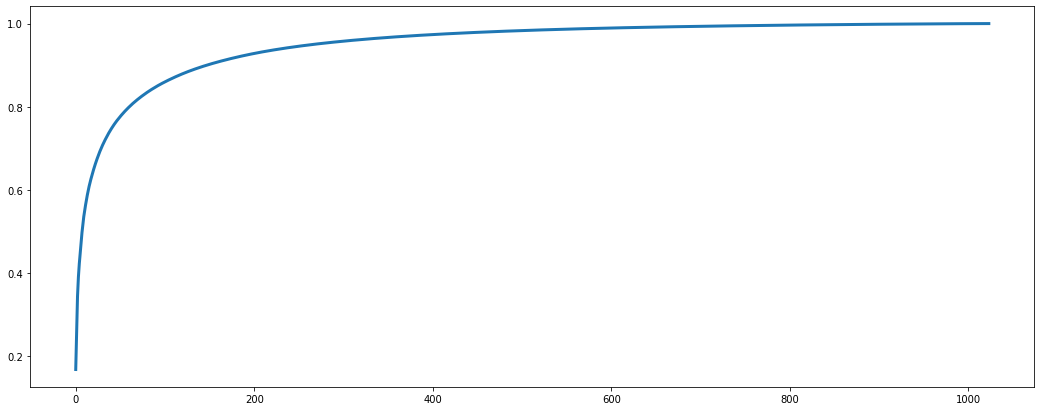
\includegraphics[width=0.6\textwidth]{Images/1.2. PCA explained_variance_ratio_cumsum.png}
    \caption{\label{fig:4.3}Explained Variance ratio cumulative sum}
\end{figure}
\noindent \\ The PCA produces 1024 eigenvectors (here called "eigenfruits") which can individually be reshaped into a 32x32 matrix and plotted (Figure \ref{fig:4.4}).\\

\begin{figure}[H]
    \centering
    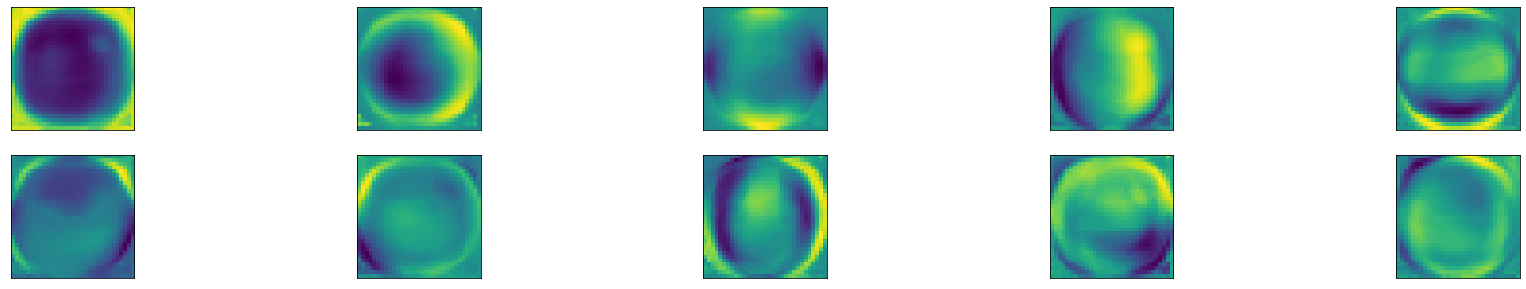
\includegraphics[width=0.7\textwidth]{Images/1.3 Eigenfruits.png}
    \caption{\label{fig:4.4}Plot of some eigenvectors ("eigenfruits")}
\end{figure}

The PCA is parametrised on the training data and its results are used to reduce the dimensionality of both training, validation, and test sets. The output for training, validation, and test is then projected onto the original space. This procedure is repeated for each of the components selected.

\begin{figure}[H]
  \centering
  \begin{minipage}[b]{0.48\textwidth}
    \centering
    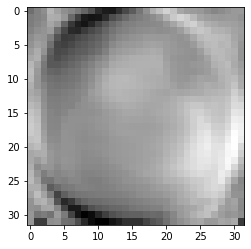
\includegraphics[width=0.25\textwidth]{Images/1.4.1 PCA 10 components image.png}
  \end{minipage}
  \hfill
  \begin{minipage}[b]{0.48\textwidth}
    \centering
    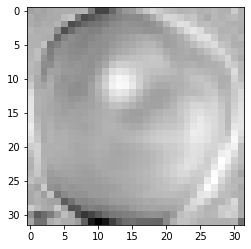
\includegraphics[width=0.25\textwidth]{Images/1.4.2 PCA 210 components image.png}
  \end{minipage}
      \caption{Image of fruit with 10 components (left) and 210 (right)}

\end{figure}
\newpage
\section{Feed Forward Neural Network}
A simple feed-forward NN is oftentimes less effective in image recognition than a convolutional neural network; however, it is still appropriate for the aim of this analysis. Indeed, it is a good starting point to evaluate if the problem can be tackled with a simple network.

The performances of the feed-forward neural networks are compared giving as input the transformed images (training, validation, test) and iterating the procedure for each set of principal components selected (i.e. 10, 30, ..., 210).

The FFNN presented in this project has a simple architecture (see Figure \ref{fig: 4.6}) and it is composed of:
\begin{itemize}
    \item one input layer with 1024 neurons corresponding to each pixel of the image;
    \item one hidden layer with 32 neurons and activation function 'relu';
    \item one output layer with 10 neurons (one for each fruit/vegetables category), with activation function 'softmax'.
\end{itemize}

Figure \ref{fig: 4.7} and Figure \ref{fig: 4.8} show accuracy and loss of training an validation sets as a function of epochs (10 epochs). The main findings are:

\begin{itemize}
    \item As expected, the training accuracy is always larger than validation accuracy given the corresponding epoch while the opposite occurs for the loss (Figure \ref{fig: 4.8});
    \item Given the epoch, accuracy and loss for the training set are almost a deterministic function of the number of components (i.e. as the number of components increases also the accuracy improves and vice versa);
    \item Given the epoch, accuracy and loss for the validation set are instead an almost deterministic function for the lowest set of components, while for a higher order of components overlappings start to occur;
    \item By measuring test error with the zero-one loss function, the optimal number of components among those tested is 170 (Figure \ref{fig: 4.9}).
\end{itemize}



\begin{figure}[H]
    \centering
    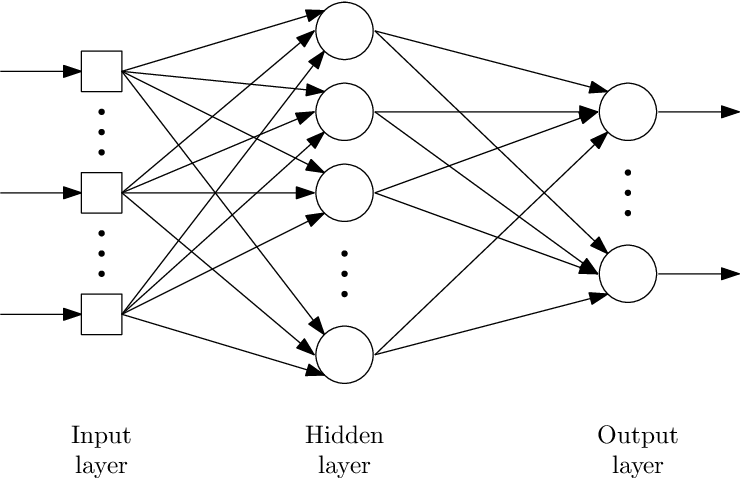
\includegraphics[width=0.5\textwidth]{Images/FFNN.png}
    \caption{\label{fig: 4.6}One-Hidden-Layer FNN}
\end{figure}



\begin{figure}[H]
    \centering
    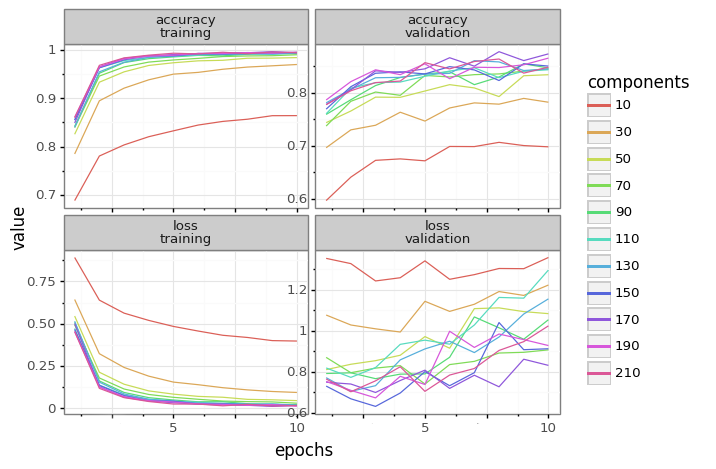
\includegraphics[width=0.7\textwidth]{Images/1.5. Accuracy and loss with different components details.png}
    \caption{\label{fig: 4.7}Accuracy and loss for training and validation set by varying the number of components given as input}
\end{figure}

\begin{figure}[H]
    \centering
    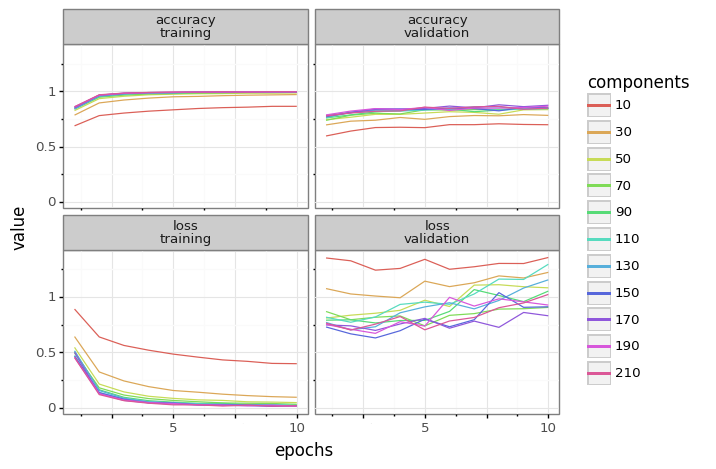
\includegraphics[width=0.7\textwidth]{Images/1.6. Accuracy and loss with different components large.png}
    \caption{\label{fig: 4.8}Large accuracy and loss plots for training and validation set by varying the number of components given as input}
\end{figure}

\clearpage
A significant reduction in loss is obtained by increasing the number of components (Figure \ref{fig: 4.9}).This is particularly true for the initial components when the slope of the curve is larger. This means that the marginal reduction in loss is larger when the number of components is low. A significant reduction is less evident after 70 components when the curve begins to plateau.

\begin{figure}[H]
    \centering
    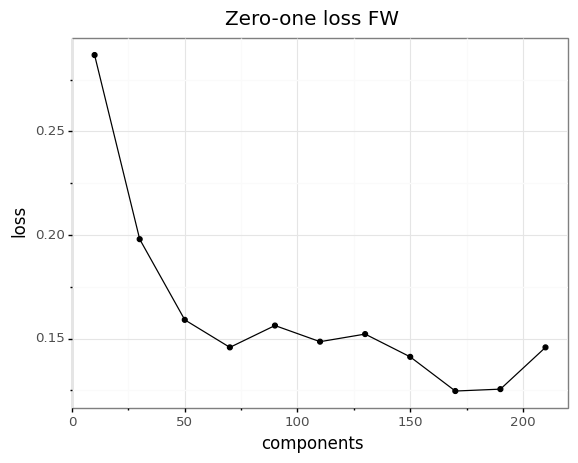
\includegraphics[width=0.5\textwidth]{Images/1.7. Test zero one loss.png}
    \caption{\label{fig: 4.9}Plot of the zero-one loss applied on test set by varying the number of components given in input}
\end{figure}

Despite being a simple neural network, giving as input to the NN data reduced with PCA, it is possible to achieve impressive results. Based on the performance on the test set, 170/190 principal components are suggested.


\chapter{Convolutional Neural Networks}\label{chapt:modelCNN}
\begin{figure}[H]
    \centering
    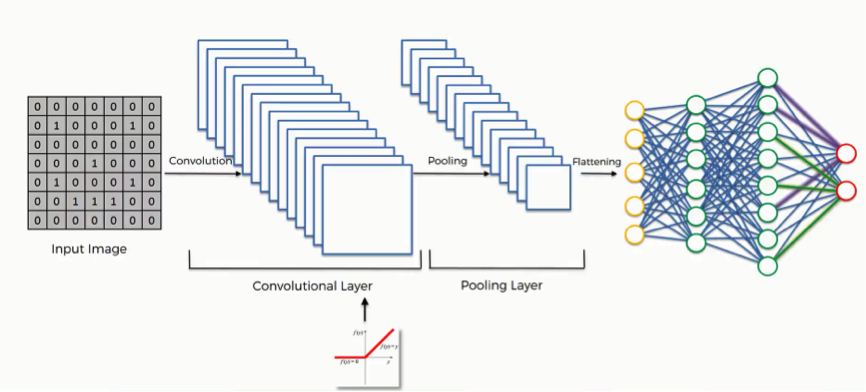
\includegraphics[width=0.8\textwidth]{Images/CNN.png}
    \caption{Generic architecture of a convolutional neural network}
\end{figure}

The aim of this chapter is to run experiments with a popular convolutional network and observe how an increase in the number of layers corresponds to an improvement or worsening of the performance if phenomena like overfitting occur.
In particular, the model implemented takes inspiration from the VGG architecture, proposed by Andrew Zisserman and Karen Simonyan in 2014.

\begin{figure}[H]
    \centering
    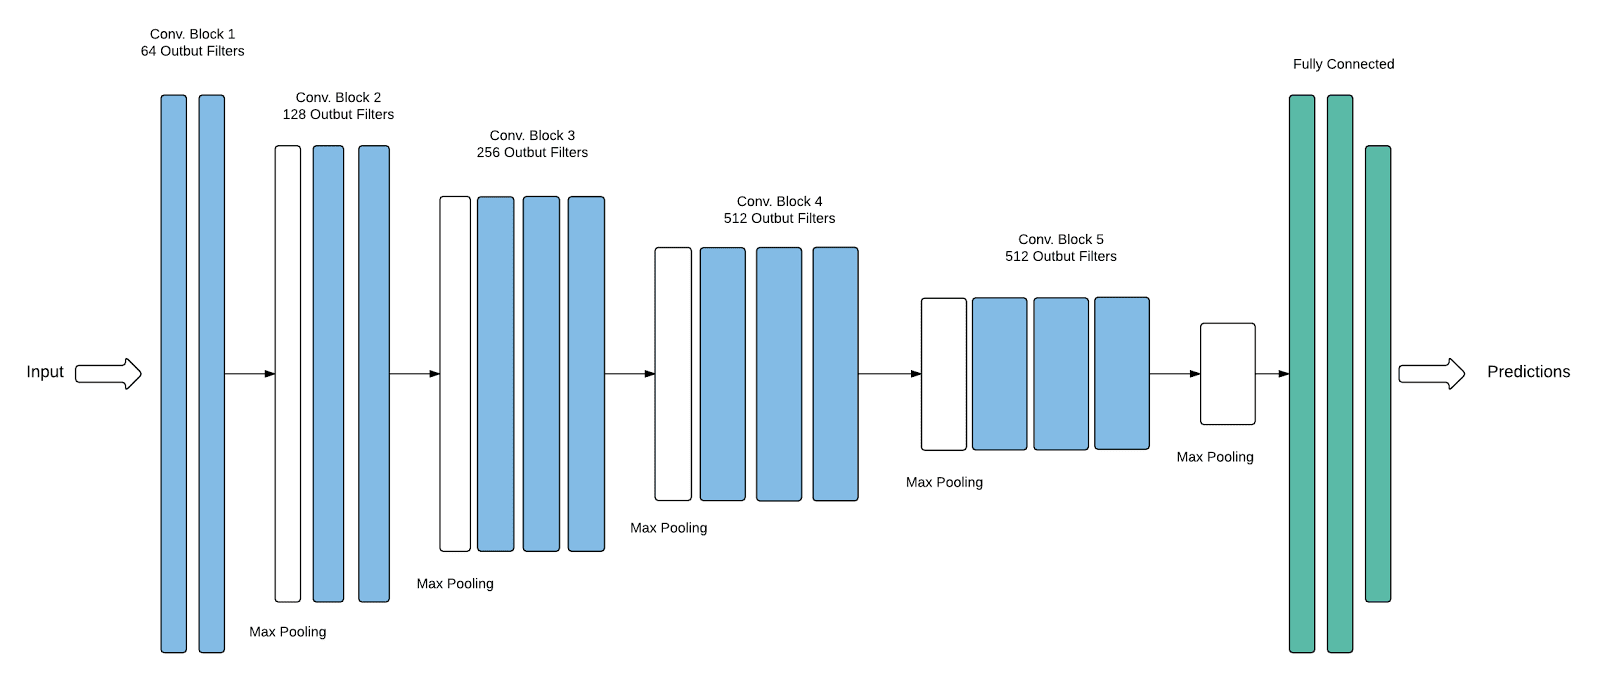
\includegraphics[width=0.7\textwidth]{Images/2.0. VGG model.png}
    \caption{VGG architecture}
\end{figure}

Different types of VGG networks are tested, progressively increasing the number of layers.

\section{VGG: one block}

\begin{verbatim}
Model: "sequential_11"
_________________________________________________________________
Layer (type)                 Output Shape              Param #   
=================================================================
conv2d (Conv2D)              (None, 32, 32, 32)        896       
_________________________________________________________________
conv2d_1 (Conv2D)            (None, 32, 32, 32)        9248      
_________________________________________________________________
max_pooling2d (MaxPooling2D) (None, 16, 16, 32)        0         
_________________________________________________________________
flatten (Flatten)            (None, 8192)              0         
_________________________________________________________________
dense_22 (Dense)             (None, 128)               1048704   
_________________________________________________________________
dense_23 (Dense)             (None, 10)                1290      
=================================================================
Total params: 1,060,138
Trainable params: 1,060,138
Non-trainable params: 0
_________________________________________________________________
\end{verbatim}



\begin{figure}[H]
    \centering
    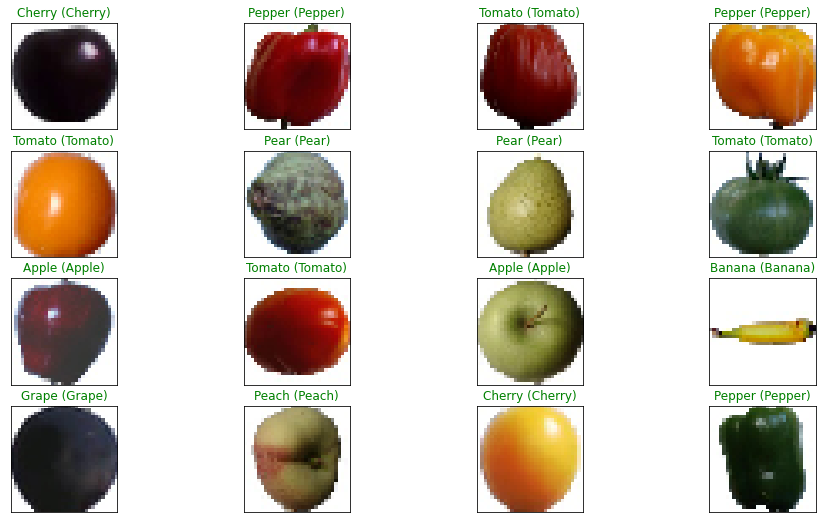
\includegraphics[width=0.6\textwidth]{Images/2.1. random predicte img VGG.png}
    \caption{Random test of the VGG-one-block CNN on the test set}
\end{figure}

\begin{figure}[H]
    \centering
    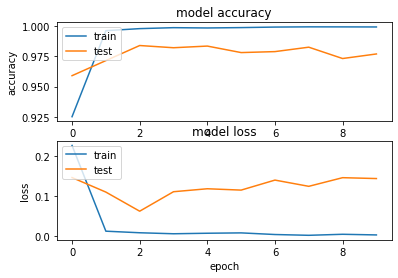
\includegraphics[width=0.7\textwidth]{Images/2.2 Accuracy Loss VGG 1.png}
    \caption{\label{fig:5.4}Accuracy and loss for training and validation of the one block VGG.}
\end{figure}

The results of Figure \ref{fig:5.4} are obtained by using a VGG architechture with a total of 6 layers whose main components are:
\begin{itemize}
    \item 2 convolutional layers
    \item a maxpooling layer
    \item a flatten layer
    \item 2 dense layers
\end{itemize}

This model learns fast in the training set and the performances on the validation are already high in the first range of epochs.
Based on the zero-one-loss, it returns a value of about 0.02 (Figure \ref{fig: 5.9}).
In the next section, the change in performance of the model is explored as more layers are introduced in the architecture (VGG two blocks).

\clearpage
\section{VGG: two blocks}


\begin{verbatim}
Model: "sequential_12"
_________________________________________________________________
Layer (type)                 Output Shape              Param #   
=================================================================
conv2d_2 (Conv2D)            (None, 32, 32, 32)        896       
_________________________________________________________________
conv2d_3 (Conv2D)            (None, 32, 32, 32)        9248      
_________________________________________________________________
max_pooling2d_1 (MaxPooling2 (None, 16, 16, 32)        0         
_________________________________________________________________
conv2d_4 (Conv2D)            (None, 16, 16, 64)        18496     
_________________________________________________________________
conv2d_5 (Conv2D)            (None, 16, 16, 64)        36928     
_________________________________________________________________
max_pooling2d_2 (MaxPooling2 (None, 8, 8, 64)          0         
_________________________________________________________________
flatten_1 (Flatten)          (None, 4096)              0         
_________________________________________________________________
dense_24 (Dense)             (None, 128)               524416    
_________________________________________________________________
dense_25 (Dense)             (None, 10)                1290      
=================================================================
Total params: 591,274
Trainable params: 591,274
Non-trainable params: 0
_________________________________________________________________
\end{verbatim}

The results of Figure \ref{fig:5.5} are obtained by using a VGG architechture with a total of 9 layers whose main components are:
\begin{itemize}
    \item 2 convolutional layers
    \item a maxpooling layer
    \item 2 convolutional layers
    \item a maxpooling layer
    \item a flatten layer
    \item 2 dense layers
\end{itemize}
\begin{figure}[H]
    \centering
    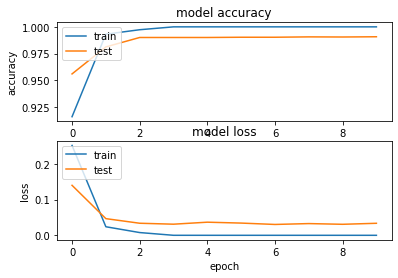
\includegraphics[width=0.7\textwidth]{Images/2.3. Accuracy loss VGG 2.png}
    \caption{ \label{fig:5.5}Accuracy and loss for training and validation of the two blocks VGG.}
\end{figure}


In Figure \ref{fig:5.5} train and validation are closer to each other compared to the previous VGG model. Furthermore, the evolution of the test accuracy as a function of epochs is more stable suggesting the presence of lower variance and higher robustness. This behaviour indicates that the model is capturing the relationship in the data more effectively than VGG one block while reducing overfitting.
The zero-one-loss returns a value of about 0.009, that shows an improvement in performance on the test set with respect to the previous model (Figure \ref{fig: 5.9}).




\newpage
\section{VGG: three blocks}

\begin{verbatim}
Model: "sequential_13"
_________________________________________________________________
Layer (type)                 Output Shape              Param #   
=================================================================
conv2d_6 (Conv2D)            (None, 32, 32, 32)        896       
_________________________________________________________________
conv2d_7 (Conv2D)            (None, 32, 32, 32)        9248      
_________________________________________________________________
max_pooling2d_3 (MaxPooling2 (None, 16, 16, 32)        0         
_________________________________________________________________
conv2d_8 (Conv2D)            (None, 16, 16, 64)        18496     
_________________________________________________________________
conv2d_9 (Conv2D)            (None, 16, 16, 64)        36928     
_________________________________________________________________
max_pooling2d_4 (MaxPooling2 (None, 8, 8, 64)          0         
_________________________________________________________________
conv2d_10 (Conv2D)           (None, 8, 8, 128)         73856     
_________________________________________________________________
conv2d_11 (Conv2D)           (None, 8, 8, 128)         147584    
_________________________________________________________________
max_pooling2d_5 (MaxPooling2 (None, 4, 4, 128)         0         
_________________________________________________________________
flatten_2 (Flatten)          (None, 2048)              0         
_________________________________________________________________
dense_26 (Dense)             (None, 128)               262272    
_________________________________________________________________
dense_27 (Dense)             (None, 10)                1290      
=================================================================
Total params: 550,570
Trainable params: 550,570
Non-trainable params: 0
_________________________________________________________________
\end{verbatim}

\begin{figure}[H]
    \centering
    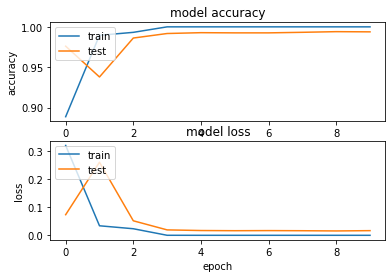
\includegraphics[width=0.7\textwidth]{Images/2.4 Accuracy Loss VGG 3.png}
    \caption{\label{fig:5.6}Accuracy and loss for training and validation of the three blocks VGG.}
\end{figure}

The results of Figure \ref{fig:5.6} are obtained by using a VGG architechture with a total of 12 layers whose main components are:
\begin{itemize}
    \item 2 convolutional layers
    \item a maxpooling layer
    \item 2 convolutional layers
    \item a maxpooling layer
    \item 2 convolutional layers
    \item a maxpooling layer
    \item a flatten layer
    \item 2 dense layers
\end{itemize}
After an anomalous peak in the first epoch, the test performance stabilises and both train and test converge as the number of epochs increases.
\newpage
\section{VGG: three blocks and Dropout}

\begin{verbatim}
Model: "sequential_14"
_________________________________________________________________
Layer (type)                 Output Shape              Param #   
=================================================================
conv2d_12 (Conv2D)           (None, 32, 32, 32)        896       
_________________________________________________________________
conv2d_13 (Conv2D)           (None, 32, 32, 32)        9248      
_________________________________________________________________
max_pooling2d_6 (MaxPooling2 (None, 16, 16, 32)        0         
_________________________________________________________________
dropout (Dropout)            (None, 16, 16, 32)        0         
_________________________________________________________________
conv2d_14 (Conv2D)           (None, 16, 16, 64)        18496     
_________________________________________________________________
conv2d_15 (Conv2D)           (None, 16, 16, 64)        36928     
_________________________________________________________________
max_pooling2d_7 (MaxPooling2 (None, 8, 8, 64)          0         
_________________________________________________________________
dropout_1 (Dropout)          (None, 8, 8, 64)          0         
_________________________________________________________________
conv2d_16 (Conv2D)           (None, 8, 8, 128)         73856     
_________________________________________________________________
conv2d_17 (Conv2D)           (None, 8, 8, 128)         147584    
_________________________________________________________________
max_pooling2d_8 (MaxPooling2 (None, 4, 4, 128)         0         
_________________________________________________________________
dropout_2 (Dropout)          (None, 4, 4, 128)         0         
_________________________________________________________________
flatten_3 (Flatten)          (None, 2048)              0         
_________________________________________________________________
dense_28 (Dense)             (None, 128)               262272    
_________________________________________________________________
dropout_3 (Dropout)          (None, 128)               0         
_________________________________________________________________
dense_29 (Dense)             (None, 10)                1290      
=================================================================
Total params: 550,570
Trainable params: 550,570
Non-trainable params: 0
_________________________________________________________________
\end{verbatim}

\begin{figure}[H]
    \centering
    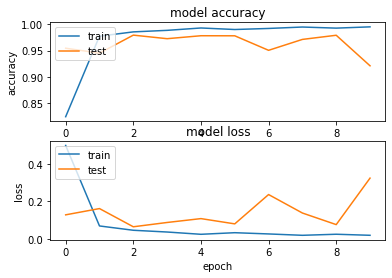
\includegraphics[width=0.7\textwidth]{Images/2.5 Accuracy Loss VGG 3 Dropout.png}
    \caption{\label{fig:5.7}Accuracy and loss for training and validation of the three blocks VGG with dropout.}
\end{figure}
\noindent \\ The results of Figure \ref{fig:5.7} are obtained by using a VGG architecture with dropout components hoping to reduce overfitting by slowing down the learning rate. The architecture consists of a total of 16 layers and it is structured as the previous one but enriched with Dropout layers.

Contrary to expectations, adding dropout layers, even if it slightly slows down the training process, results in a worse performance than in the previous model on the test set and loss and accuracy appear less stable as the number of epochs increases. To increase performance and stability of the neural network, in next section, dropout layers are combined with batch normalisation.
\newpage
\section{VGG: three blocks with Dropout and Batch Normalization}

\begin{verbatim}
Model: "sequential_15"
_________________________________________________________________
Layer (type)                 Output Shape              Param #   
=================================================================
conv2d_18 (Conv2D)           (None, 32, 32, 32)        864       
_________________________________________________________________
batch_normalization (BatchNo (None, 32, 32, 32)        128       
_________________________________________________________________
activation (Activation)      (None, 32, 32, 32)        0         
_________________________________________________________________
conv2d_19 (Conv2D)           (None, 32, 32, 32)        9216      
_________________________________________________________________
batch_normalization_1 (Batch (None, 32, 32, 32)        128       
_________________________________________________________________
activation_1 (Activation)    (None, 32, 32, 32)        0         
_________________________________________________________________
max_pooling2d_9 (MaxPooling2 (None, 16, 16, 32)        0         
_________________________________________________________________
dropout_4 (Dropout)          (None, 16, 16, 32)        0         
_________________________________________________________________
conv2d_20 (Conv2D)           (None, 16, 16, 64)        18432     
_________________________________________________________________
batch_normalization_2 (Batch (None, 16, 16, 64)        256       
_________________________________________________________________
activation_2 (Activation)    (None, 16, 16, 64)        0         
_________________________________________________________________
conv2d_21 (Conv2D)           (None, 16, 16, 64)        36864     
_________________________________________________________________
batch_normalization_3 (Batch (None, 16, 16, 64)        256       
_________________________________________________________________
activation_3 (Activation)    (None, 16, 16, 64)        0         
_________________________________________________________________
max_pooling2d_10 (MaxPooling (None, 8, 8, 64)          0         
_________________________________________________________________
dropout_5 (Dropout)          (None, 8, 8, 64)          0         
_________________________________________________________________
conv2d_22 (Conv2D)           (None, 8, 8, 128)         73728     
_________________________________________________________________
batch_normalization_4 (Batch (None, 8, 8, 128)         512       
_________________________________________________________________
activation_4 (Activation)    (None, 8, 8, 128)         0         
_________________________________________________________________
conv2d_23 (Conv2D)           (None, 8, 8, 128)         147456    
_________________________________________________________________
batch_normalization_5 (Batch (None, 8, 8, 128)         512       
_________________________________________________________________
activation_5 (Activation)    (None, 8, 8, 128)         0         
_________________________________________________________________
max_pooling2d_11 (MaxPooling (None, 4, 4, 128)         0         
_________________________________________________________________
dropout_6 (Dropout)          (None, 4, 4, 128)         0         
_________________________________________________________________
flatten_4 (Flatten)          (None, 2048)              0         
_________________________________________________________________
dense_30 (Dense)             (None, 128)               262144    
_________________________________________________________________
batch_normalization_6 (Batch (None, 128)               512       
_________________________________________________________________
activation_6 (Activation)    (None, 128)               0         
_________________________________________________________________
dropout_7 (Dropout)          (None, 128)               0         
_________________________________________________________________
dense_31 (Dense)             (None, 10)                1290      
=================================================================
Total params: 552,298
Trainable params: 551,146
Non-trainable params: 1,152
_________________________________________________________________
\end{verbatim}

\begin{figure}[H]
    \centering
    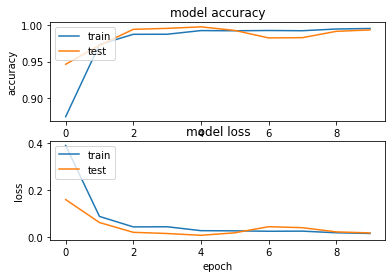
\includegraphics[width=0.7\textwidth]{Images/2.6. Accuracy Loss VGG Drop BN.png}
    \caption{\label{fig:5.8}Accuracy and loss for training and validation of the three blocks VGG with Batch Normalization.}
\end{figure}
\newpage
The results of Figure \ref{fig:5.8} are obtained by using a VGG architecture with a total of 30 layers where batch normalization layers are added (as shown in the summary table).
Performance on the validation set improves compared to the previous VGG models and in some epochs it is even better than the training accuracy/loss. As previously mentioned, the goal of models with dropout is to slow down the learning curve because this function randomly drops the connections between some neurons during the training phase. Even if a slowdown in the learning rate is less obvious it is still noticeable. Perhaps a reason for this is that, without a dropout layer, 100\% accuracy in the training set can already be achieved in epochs 3/4 whereas models with dropout never reach 100\% accuracy but they asymptotically tend towards it. A possible reason why validation performance is higher that training performance is that using dropout layers in the training process some neurons are randomly deactivated whereas during validation all of the units are available so the network has its full computational power and thus it might perform better than in training.
\\
\begin{figure}[H]
    \centering
    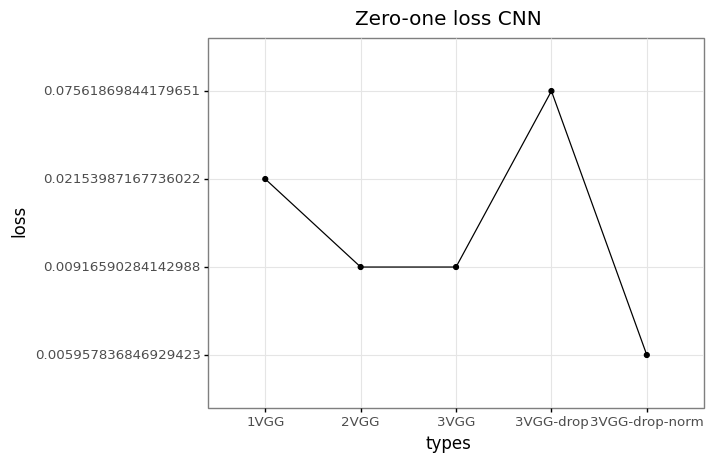
\includegraphics[width=0.7\textwidth]{Images/2.7. Test Zero One loss VGG.png}
    \caption{\label{fig: 5.9}Zero one Loss on test set for each VGG architecture}
\end{figure}
\noindent \\
According to the zero-one loss, Figure \ref{fig: 5.9} shows that 3VGG with dropout and batch normalisation has overall the best performance. However, all the models give satisfactory results.

\chapter{Examples of famous CNN architectures: LeNet and MobileNetV2}\label{chapt:modelCNN2}

VGG and PCA with one hidden layer feed-forward already give satisfactory results to solve this classification problem. However, it is worth exploring whether mainstream models with architectures openly shared online like LeNet and MobileNetV2 perform better.

\section{LeNet Architecture}

LeNet is a convolutional neural network structure proposed by Yann LeCun et al. in 1998, originally  applied to the recognition of handwritten zip code digits provided by the U.S. Postal Service. 
It is a simple convolutional neural network (7-layers), that includes the classical features of convolutional neural networks such as convolutional layers, pooling layers and full connection layers.

\begin{figure}[H]
    \centering
    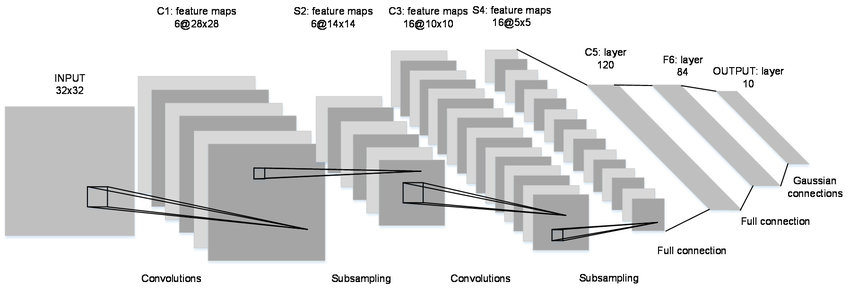
\includegraphics[width=0.7\textwidth]{Images/3.0. LeNet.png}
    \caption{LeNet Architecture}
\end{figure}

\begin{figure}[H]
    \centering
    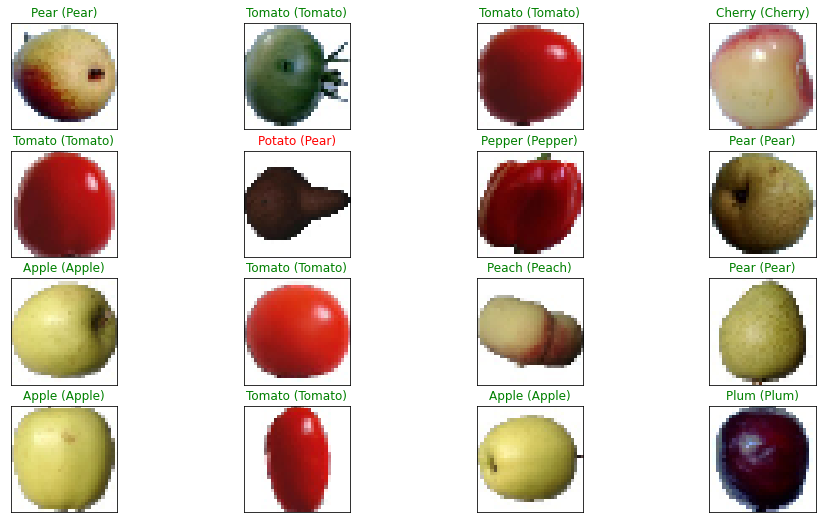
\includegraphics[width=0.7\textwidth
]{Images/3.1. LeNet random images prediction.png}
    \caption{Random test of LeNet architecture on test set}
\end{figure}

\begin{figure}[H]
    \centering
    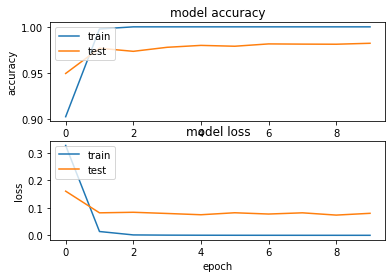
\includegraphics[width=0.7\textwidth]{Images/3.2. Accuracy loss Lenet.png}
    \caption{Accuracy and loss function of LeNet architecture}
\end{figure}

LeNet offers a suitable performance and a stable solution without obvious evidence of overfitting. Due to the simplicity of the problem, the model learns rapidly and outputs a fairly accurate classification in the validation set already starting from the first epoch.

\section{MobileNetV2 Architecture}

MobileNetV2 was introduced by Google in 2019 and is an evolution of a previous architecture called MobileNetV1. Experimenting with this architecture is an interesting research task and it is an opportunity to test a more recent and complex model. MobileNetV2 was optimised to run with machines with a discrete computational power (despite its complexity) such as mobile devices.

\begin{figure}[H]
    \centering
    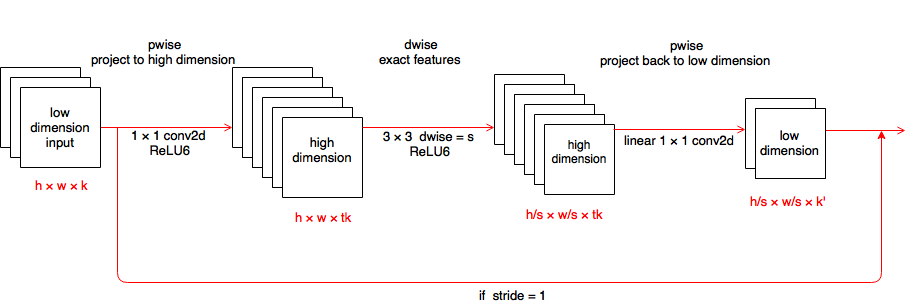
\includegraphics[width=0.8\textwidth]{Images/MobileNetV2.png}
    \caption{MobileNetV2 Architecture}
\end{figure}

\begin{figure}[H]
    \centering
    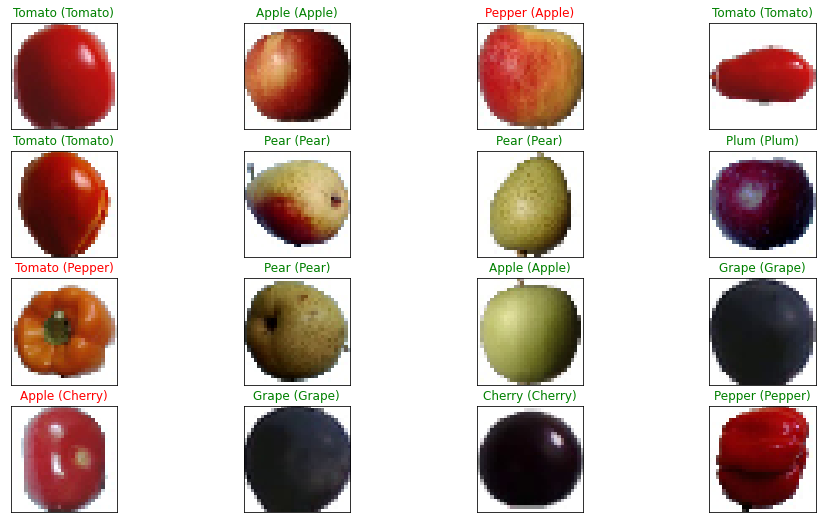
\includegraphics[width=0.6\textwidth]{Images/3.3. MobileNetV2 random images prediction.png}
    \caption{\label{fig:6.5}Random test of MobileNetV2 architecture on test set}
\end{figure}


\begin{figure}[H]
    \centering
    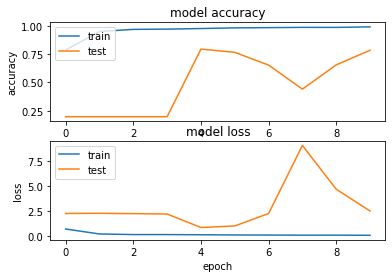
\includegraphics[width=0.7\textwidth]{Images/3.4. Accuracy Loss MobileNetv2.png}
    \caption{Accuracy and loss function of LeNet architecture}
\end{figure}
\noindent \\ The results of MobileNetV2 on this classification problem are not promising. Indeed, the algorithm learns quickly on the training set and it is not reliable on the validation set. Evidence suggests it is a case of overfitting and the architecture is presumably too complex for this classification problem. Figure \ref{fig:6.5} shows an application of the algorithm on a random sample of 16 images from the test set that returns a classification error of 3 wrong images out of 16.

\chapter{Conclusion}\label{chapt:results}
\begin{figure}[H]
    \centering
    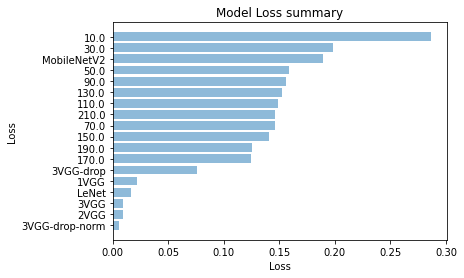
\includegraphics[width=0.6\textwidth]{Images/4. Models ranking.png}
    \caption{\label{fig:7.1}Models ranking}
\end{figure}

Figure \ref{fig:7.1} illustrates a ranking of the performance of the architectures explored in this research, according to the zero-one loss function.

Overall, the model that returns the best solution for the problem is the 3 layers VGG architecture with Dropout and Batch normalization, followed by the other VGG networks without Dropout and the LeNet network.
As concerns the one hidden layer feed-forwards NNs with PCA, also 170 an 190 components offer a fairly good solution, having a loss approximately equal to 0.12 (a good complexity/performance trade-off).

In the light of the findings and observations of this research, it can be concluded that:

\begin{itemize}
    \item Experimenting with simpler neural networks first and progressively expanding their complexity can be a good strategy to identify an optimal fit among the architectures available
    \item Neural networks do not necessarily need all the variance in the data to effectively classify images. Some residual variance can be considered as noise for the model and actually make it more difficult for the neural network to predict categories. In this regard, PCA can be an appropriate technique to reduce the noise of the input images and facilitate the problem.
    \item A higher complexity does not necessarily imply a higher performance: it is necessary to calibrate the complexity of the network to the problem we are presented with to avoid overfitting/underfitting problems (i.e. parsimonious modelling).
    \item In case the marginal learning rate is too high, dropout techniques and batch normalisation can be introduced to favour an improved learning and generalisability of the problem.
\end{itemize}

\chapter{Bibliography}\label{chapt:bibliografy}
%\bibliographystyle{plain}
%\bibliography{bibliography.bib}
\printbibliography

Dataset: https://www.kaggle.com/moltean/fruits \\ \\
Zero- one loss image: https://www.researchgate.net/figure/The-function-s-a-z-is-a-soft-differentiable-approximation-of-the-zero-one-loss-The\_fig1\_230679870 \\ \\
https://www.researchgate.net/figure/The-LeNet-5-Architecture-a-convolutional-neural-network\_fig4\_321586653
       paper: LeCun, Y.; Boser, B.; Denker, J. S.; Henderson, D.; Howard, R. E.; Hubbard, W. \& Jackel, L. D. (1989). Backpropagation applied to handwritten zip code recognition.
\\ \\
https://www.codesofinterest.com/p/build-deeper.html
     paper: Simonyan, K.; Zisserman A. (2015).  Very Deep Convolutional Networks for Large-Scale Image Recognition. 
\\\\
https://awesomeopensource.com/project/ShuangXieIrene/mobilenet-v2
	 paper: Krizhevsky, A.; Sutskever, I.; Hinton, G. (2010). ImageNet Classification with Deep Convolutional Neural Networks.
\\\\
CNN image: https://www.superdatascience.com/blogs/convolutional-neural-networks-cnn-summary/



\end{document}
